\section{Users}

Die Nutzerseite erlaubt es, registrierten Nutzern im Sokka-System eine Rabattgruppe zuzweisen oder sie komplett aus der Datenbank zu entfernen. In der Suchleiste kann nach Nutzer-E-Mail gefiltert werden.

\begin{figure}[ht]
    \centering
    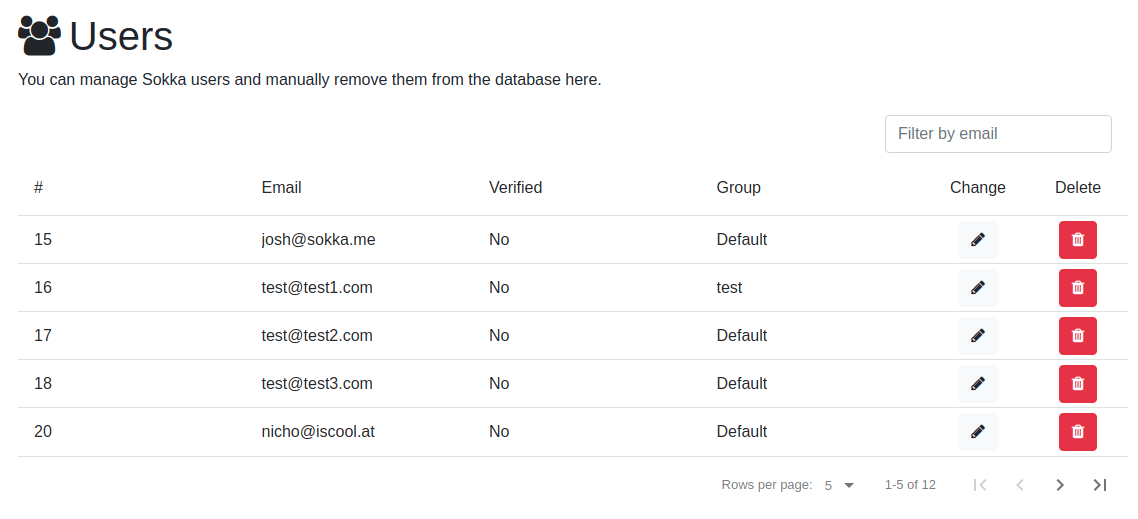
\includegraphics[width=0.8\textwidth]{images/ACP/users-page.png}
    \caption{Die Nutzerseite des Sokka-ACPs}
\end{figure}

\textbf{\#} ist die interne und eindeutige Nutzer-ID, \textbf{E-Mail} die vom Nutzer angegebene E-Mail-Adresse, \textbf{Verified} ist der Status der Verifizierung des Nutzers (genaueres in Sektion \textit{\glqq\nameref{verification}\grqq} im Backend-Teil), \textbf{Group} die festgelegte Rabattgruppe (standardmäßig \textit{Default}) und Change bzw. Delete sind Aktionsspalten.

Der \textit{Change}-Button in jeder Zeile erlaubt das Ändern der Rabattgruppe eines Nutzers. Rabattgruppen müssen zuerst im Reiter \textit{\glqq\nameref{acp-groups}\grqq} konfiguriert werden. Danach können erstellte Gruppen im Change-Dialog ausgewählt werden.

\begin{figure}[ht]
    \centering
    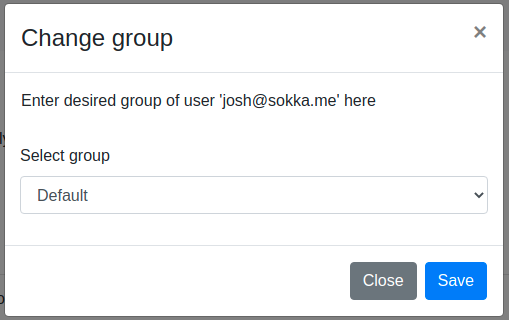
\includegraphics[width=0.6\textwidth]{images/ACP/users_modal.png}
    \caption{Der Dialog zum Ändern von Rabattgruppen von Nutzern im Sokka-ACP}
\end{figure}